\begin{frame}
    \frametitle{Particle Filter}
    \note{Content from Cyrill Stachniss's video: https://youtu.be/MsYlueVDLI0}
    \footnotesize
    \begin{itemize}
        \item EKF is limited to Gaussian distributions
        \item With EKF we obtain a Gaussian distribution describing the robot's location
        \item Particle Filters use particles/hypotheses representing possible robot positions
        \item Instead of parametric forms (like EKF with mean $\mu$ and covariance $\covariance$), Particle Filters use non-parametric samples as hypotheses
    \end{itemize}
    
    \begin{center}
        \movie[loop]{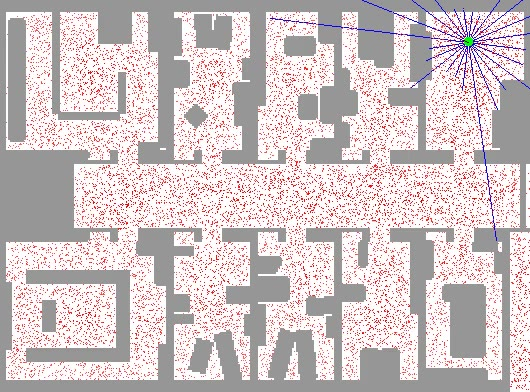
\includegraphics[width=0.4\columnwidth]{images/particle_filter/particle_filter_video.jpg}}{videos/particle_filter.mp4}
    \end{center}
    
    \note{Video from https://rse-lab.cs.washington.edu/projects/mcl/animations/global-floor.gif}
\end{frame}

\begin{frame}
    \frametitle{Flexible Function Approximation}
    \note{Content from Cyrill Stachniss's video: https://youtu.be/MsYlueVDLI0}
    \footnotesize
    
    \begin{itemize}
        \item Goal: Approach that allows estimating any \textbf{arbitrary probability distribution}
    \end{itemize}
    
    \begin{center}
    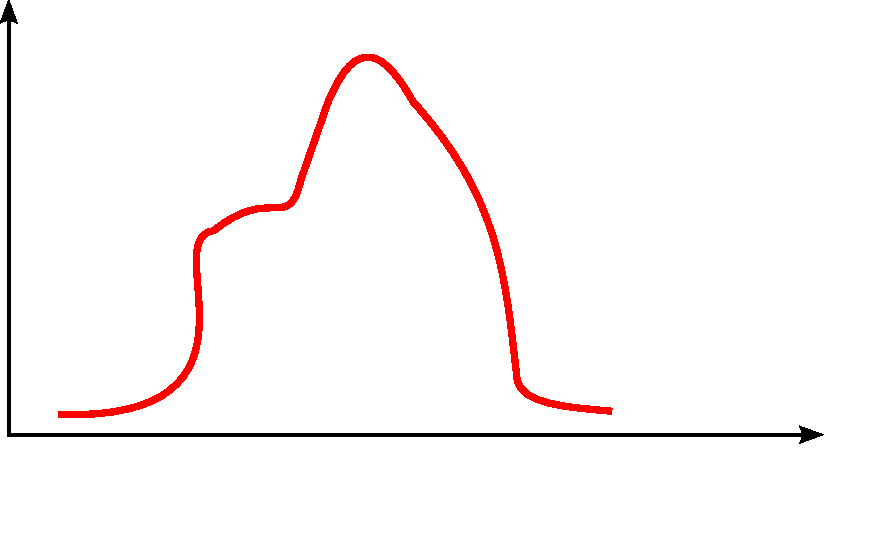
\includegraphics[width=0.5\columnwidth]{./images/particle_filter/arbitrary_distribution.pdf}
    \end{center}
\end{frame}

\begin{frame}
    \frametitle{Using Samples (Particles)}
    \note{Content from Cyrill Stachniss's video: https://youtu.be/MsYlueVDLI0}
    \footnotesize
    \begin{itemize}
        \item \textbf{Multiple samples} to represent an arbitrary probability distribution
        \item Samples cluster in some areas more than others - density indicates likelihood
        \item Each sample accumulates "probability mass"
        \item Samples approximate the probability density function (pdf)
        \item To get the pdf, integrate over an area to obtain the probability mass
        \item More particles where pdf is high, fewer where low
    \end{itemize}
    
    \begin{center}
    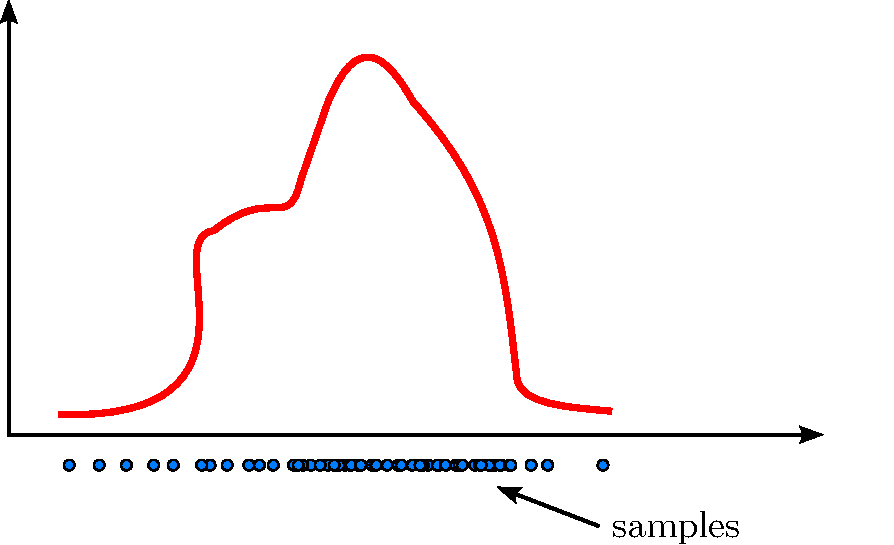
\includegraphics[width=0.5\columnwidth]{./images/particle_filter/arbitrary_distribution_samples.pdf}
    \end{center}
\end{frame}

\begin{frame}
    \frametitle{Using Weighted Samples}
    \note{Content from Cyrill Stachniss's video: https://youtu.be/MsYlueVDLI0}
    \footnotesize
    \begin{itemize}
        \item Alternative: Use \textbf{weighted samples} to reduce required particle count
        \item Higher weight indicates more probability mass in that region
        \item All weights must sum to 1
        \item Initially, uniform weights can be assigned (e.g., $1/n$ for $n$ samples)
    \end{itemize}
    
    \begin{center}
        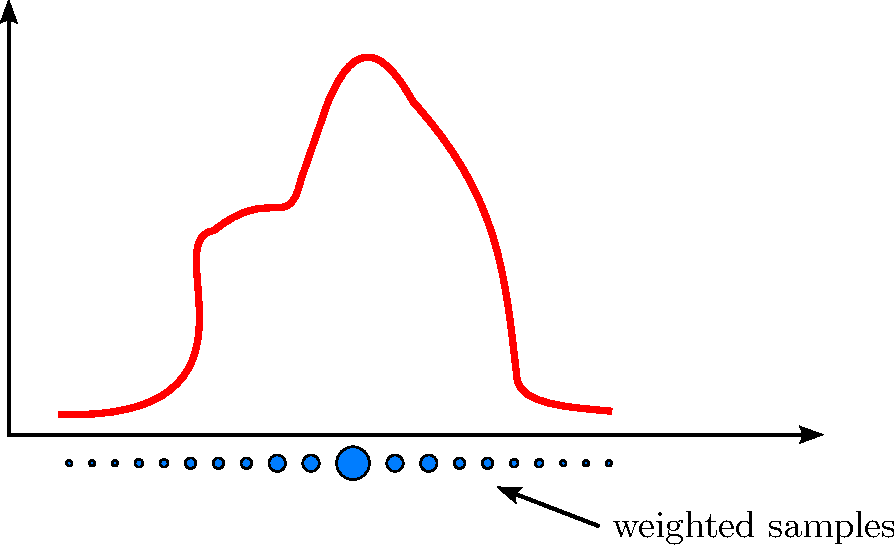
\includegraphics[width=0.5\columnwidth]{./images/particle_filter/arbitrary_distribution_weighted_samples.pdf}
    \end{center}
\end{frame}

\begin{frame}
    \frametitle{Particle Filter}
    \note{Content from Cyrill Stachniss's video: https://youtu.be/MsYlueVDLI0}
    \footnotesize
    \begin{itemize}
        \item Note this is an approximation of the PDF (Probability Density Function)
        \item Sufficient samples are needed to properly represent the PDF
    \end{itemize}
\end{frame}

\begin{frame}
    \frametitle{Particle Set}
    \note{Content from Cyrill Stachniss's video: https://youtu.be/MsYlueVDLI0}
    
    \begin{itemize}
        \item Weighted particle set:
            
        \begin{center}
            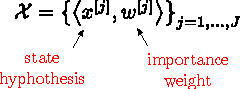
\includegraphics[width=0.5\columnwidth]{./images/particle_filter/weighted_samples.pdf}
        \end{center}

        \item Particles represent the posterior belief:
        \begin{equation*}
            p(x) = \sum_{j=1}^{J} w^{[j]} \delta_{x^{[j]}}(x)    
        \end{equation*}
        where $\delta_{x^{[j]}}(x)$ is the Dirac delta centered at particle $x^{[j]}$

        \begin{equation*}
            \delta(y) = 
            \begin{cases} 
            \infty, & y = x^{[j]} \\ 
            0, & y \neq x^{[j]} 
            \end{cases}    
        \end{equation*}

        \note{The Dirac delta models impulses/events}
        \note{More particles are needed for more complex pdfs}
    \end{itemize}
\end{frame}

\begin{frame}
    \frametitle{Particles for Approximation}
    \note{Content from Cyrill Stachniss's video: https://youtu.be/MsYlueVDLI0}
    
    \begin{itemize}
        \item Particles approximating a function
        
        \begin{center}
            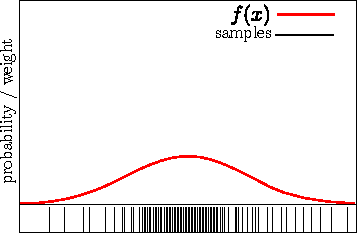
\includegraphics[width=0.45\columnwidth]{./images/particle_filter/gaussian_approximation_by_sampling.pdf}
            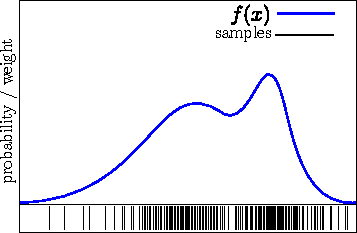
\includegraphics[width=0.45\columnwidth]{./images/particle_filter/particles_for_approximation.pdf}
        \end{center}

        \item More particles in a region indicates higher probability
    \end{itemize}
    
    \begin{center}
        \alert{How to obtain these samples?}
    \end{center}

    \note{Closed-form sampling is only possible for few distributions}
\end{frame}

\begin{frame}
    \frametitle{Closed-Form Sampling is Only Possible for Few Distributions}
    \note{Content from Cyrill Stachniss's video: https://youtu.be/MsYlueVDLI0}

    \begin{itemize}
        \item Example: Sampling from a Gaussian Distribution
    \end{itemize}

    \begin{figure}
        \begin{minipage}[m]{.5\textwidth}
            \raggedright
            \begin{center}
                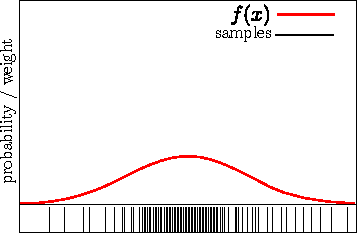
\includegraphics[width=\columnwidth]{./images/particle_filter/gaussian_approximation_by_sampling.pdf}
            \end{center}
        \end{minipage}%
        \begin{minipage}[m]{.5\textwidth}
            \raggedleft
            \centering
            \begin{equation*}
                x \leftarrow \frac{1}{2} \sum_{i=1}^{12} \text{rand}(-\sigma, \sigma)    
            \end{equation*}
        \end{minipage}
    \end{figure}

    How to sample using other distributions?

    \note{Importance Sampling Principle technique}
\end{frame}

\begin{frame}
    \frametitle{Importance Sampling Principle}
    \note{Content from Cyrill Stachniss's video: https://youtu.be/MsYlueVDLI0}

    \scriptsize

    \begin{itemize}
        \item We can use a different distribution $\pi$ to generate samples from target distribution $f$
        \item Compensate differences using weights $w = f(x) / \pi(x)$
        \item Target distribution $f$
        \item Proposal distribution $\pi$
        \item Precondition: $f(x) > 0 \implies \pi(x) > 0$
        
        \begin{center}
        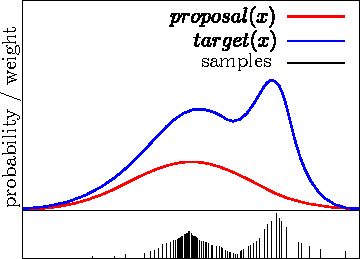
\includegraphics[width=0.4\textwidth]{./images/particle_filter/importance_sampling_principle.pdf}
        \end{center}
        
        Larger differences between target and proposal yield higher weights
    \end{itemize}
\end{frame}

\begin{frame}
    \frametitle{Particle Filter for Dynamic State Estimation}
    \note{Content from Cyrill Stachniss's video: https://youtu.be/MsYlueVDLI0}

    \begin{itemize}
        \item Implements Recursive Bayesian Filter (prediction + correction steps)
        \item Non-parametric approach (handles non-Gaussian distributions)
        \item Models distribution through samples
        \item \textbf{Prediction}: Sample from proposal distribution
        \item \textbf{Correction}: Weight by target/proposal ratio
        \item \alert{More samples yield better estimates!}
    \end{itemize}
\end{frame}

\begin{frame}
    \frametitle{Particle Filter Algorithm}
    \note{Content from Cyrill Stachniss's video: https://youtu.be/MsYlueVDLI0}

    \begin{enumerate}
        \item Sample particles using proposal distribution:
        \begin{equation*}
            x_{t}^{[j]} \sim \pi(x_t) 
        \end{equation*}
        \item Compute importance weights:
        \begin{equation*}
            w_t^{[j]} = \frac{p(x_t^{[j]})}{\pi(x_t^{[j]})}
        \end{equation*}
        \item Resampling: Select particle $i$ with probability $\propto w_t^{[j]}$, repeat $J$ times
    \end{enumerate}

    Connection to Recursive Bayesian Filter:
    \begin{itemize}
        \item Step 1: Prediction using motion model
        \item Steps 2-3: Correction using observation model
    \end{itemize}
\end{frame}

\begin{frame}
    \frametitle{Particle Filter Algorithm}
    \note{Content from Cyrill Stachniss's video: https://youtu.be/MsYlueVDLI0}

    \begin{algorithmic}[1]
    \Procedure{ParticleFilter}{$\mathcal{X}_{t-1}, u_{t}, z_{t}$}
    \State $\bar{\mathcal{X}}_t = \mathcal{X}_t = \emptyset$
    \For{$j = 1$ to $J$}
        \State sample $x_t^{[j]} \sim \pi(x_t)$
        \State $w_t^{[j]} = \dfrac{p(x_t^{[j]})}{\pi(x_t^{[j]})}$
        \State $\bar{\mathcal{X}}_t = \bar{\mathcal{X}}_t + \langle x_t^{[j]}, w_t^{[j]}\rangle$
    \EndFor
    \For{$j = 1$ to $M$}
        \State Draw $i$ with probability $\propto w_t^{[i]}$
        \State Add $x_t^{[i]}$ to $\mathcal{X}_t$
    \EndFor
    \State return $\mathcal{X}_t$
    \EndProcedure
    \end{algorithmic}
\end{frame}

\begin{frame}
    \frametitle{Monte Carlo Localization}
    \note{Content from Cyrill Stachniss's video: https://youtu.be/MsYlueVDLI0}

    Monte Carlo Localization: Particle Filter for robot localization
\end{frame}

\begin{frame}
    \frametitle{Monte Carlo Localization}
    \note{Content from Cyrill Stachniss's video: https://youtu.be/MsYlueVDLI0}

    \begin{itemize}
        \item Each particle is a pose hypothesis
        \item Proposal is motion model:
        \begin{equation*}
            x_t^{[j]} \sim p(x_t | x_{t-1}, u_t)
        \end{equation*}
        \item Correction via observation model:
        \begin{equation*}
            w_t^{[j]} \propto p(z_t | x_t, m)
        \end{equation*}
    \end{itemize}
\end{frame}

\begin{frame}
    \frametitle{Particle Filter for Localization}
    \note{Content from Cyrill Stachniss's video: https://youtu.be/MsYlueVDLI0}

    \begin{algorithmic}[1]
        \Procedure{ParticleFilter}{$\mathcal{X}_{t-1}, u_t, z_t$}
        \State $\bar{\mathcal{X}}_t = \mathcal{X}_t = \emptyset$
        \For{$j = 1$ to $J$}
            \State Sample $x_t^{[j]} \sim p(x_t | u_t, x_{t-1}^{[j]})$
            \State $w_t^{[j]} = p(z_t | x_t^{[j]})$
            \State $\bar{\mathcal{X}}_t = \bar{\mathcal{X}}_t + \langle x_t^{[j]}, w_t^{[j]}\rangle$
        \EndFor
        \For{$i = 1$ to $J$}
            \State Draw $i \in 1,\ldots,J$ with probability $\propto w_t^{[i]}$
            \State Add $x_t^{[i]}$ to $\mathcal{X}_t$
        \EndFor
        \State return $\mathcal{X}_t$
    \EndProcedure
    \end{algorithmic}
\end{frame}

\begin{frame}
    \frametitle{Resampling}
    \note{Content from Cyrill Stachniss's video: https://youtu.be/MsYlueVDLI0}

    \begin{itemize}
        \item Select particle $i$ with probability $\propto w_t^{[i]}$, repeat $J$ times
        \item "Replace unlikely samples with more probable ones"
        \item Survival of the fittest
        \item Prevents wasting samples on low-probability states
        \item Necessary due to finite memory (limited particles)
    \end{itemize}
\end{frame}

\begin{frame}
    \frametitle{Resampling Methods}
    \note{Content from Cyrill Stachniss's video: https://youtu.be/MsYlueVDLI0}

    \scriptsize

    \begin{overlayarea}{\textwidth}{\textheight}
        \only<1>{
            \begin{center}
                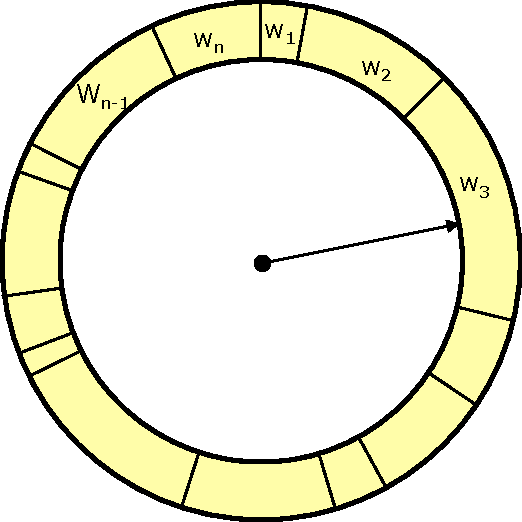
\includegraphics[width=0.3\textwidth]{./images/particle_filter/resampling_rulette_wheel1.pdf}
            \end{center}
        }
        \only<2>{
            \begin{center}
                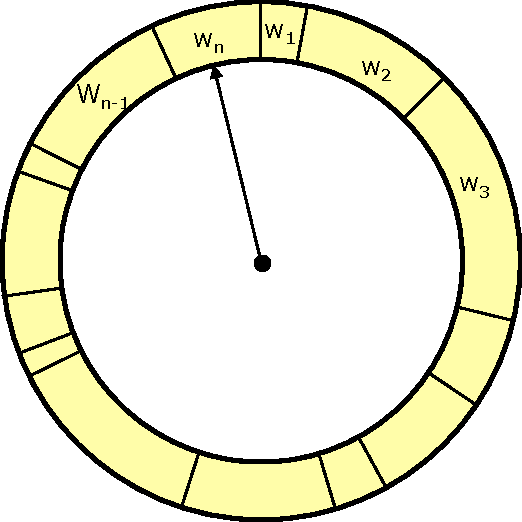
\includegraphics[width=0.3\textwidth]{./images/particle_filter/resampling_rulette_wheel2.pdf}
            \end{center}
        }
        \only<3>{
            \begin{center}
                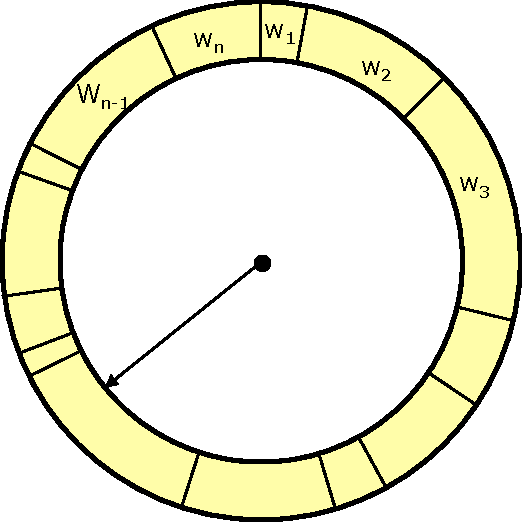
\includegraphics[width=0.3\textwidth]{./images/particle_filter/resampling_rulette_wheel3.pdf}
            \end{center}
        }
        \begin{itemize}
            \item Roulette Wheel
            \item Bucket size corresponds to particle weight
            \item Requires $J$ selections
            \item Binary search determines selected bucket ($O(J \log J)$)
        \end{itemize}
    \end{overlayarea}
\end{frame}

\begin{frame}
    \frametitle{Resampling Methods}
    \note{Content from Cyrill Stachniss's video: https://youtu.be/MsYlueVDLI0}

    \footnotesize

    \begin{overlayarea}{\textwidth}{\textheight}
        \only<1>{
            \begin{center}
                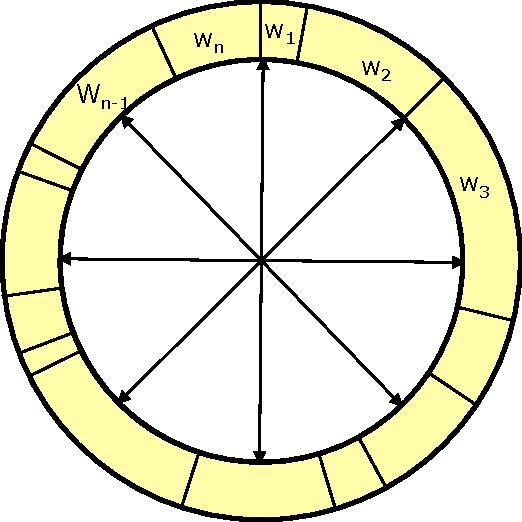
\includegraphics[width=0.3\textwidth]{./images/particle_filter/resampling_stochastic_universal_sampling1.pdf}
            \end{center}
        }
        \only<2>{
            \begin{center}
                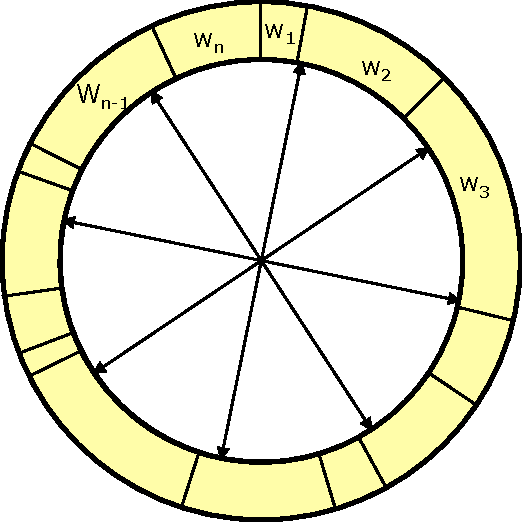
\includegraphics[width=0.3\textwidth]{./images/particle_filter/resampling_stochastic_universal_sampling2.pdf}
            \end{center}
        }

        \begin{itemize}
            \item Stochastic Universal Sampling (using $J$ equidistant arrows)
            \item Also called Low-Variance Resampling
            \item Linear computational cost $O(J)$
        \end{itemize}
    \end{overlayarea}
\end{frame}


\begin{frame}
    \frametitle{Low Variance Resampling}
    \begin{algorithmic}[1]
        \Procedure{LowVarianceResampling}{$\mathcal{X}_{t}$, $\mathcal{W}_{t}$}
        \State $\bar{\mathcal{X}}_t = \emptyset$
        \State $r = \text{rand}(0; J^{-1})$
        \State $c = w_t^{[1]}$
        \State $i = 1$
        \For{$j = 1$ to $J$}
            \State $U = r + (j - 1) J^{-1}$
            \While{$U > c$}
                \State $i = i + 1$
                \State $c = c + w_t^{[i]}$
            \EndWhile
            \State Add $x_t^{[i]}$ to $\bar{\mathcal{X}}_t$
        \EndFor
        \State Return $\bar{\mathcal{X}}_t$
        \EndProcedure
    \end{algorithmic}
\end{frame}

\begin{frame}
    \frametitle{Low Variance Resampling}
    \note{Information extracted from Cyrill Stachniss' video https://youtu.be/MsYlueVDLI0}
    \begin{itemize}
        \item Performs resampling that preserves samples when they have equal weights.
        \item Faster than Roulette Wheel resampling: $\mathcal{O}(J)$ vs. $\mathcal{O}(J \log J)$.
        \item \alert{We will always use Low Variance Resampling!}
    \end{itemize}
\end{frame}

\begin{frame}
    \frametitle{Disadvantages of Particle Filter}
    \note{Information extracted from Cyrill Stachniss' video https://youtu.be/MsYlueVDLI0}
    \begin{itemize}
        \item Does not scale well for high-dimensional spaces.
        \note{PF becomes computationally expensive because many particles are needed to cover the probability distribution. PF works well for low dimensions, up to 4, but beyond that, heuristics are needed to reduce the number of particles while keeping them representative.}
        \note{The number of particles grows exponentially with the state dimensions.}
        \item Problematic in situations with high uncertainty.
        \item \emph{Depletion Problem} (most particles have low weight).
        \note{The Depletion Problem: occurs when we have too few particles relative to the state dimensionality. The particles do not cover high-probability areas, causing them to "die" and the filter to eventually diverge.}
        \note{Example: Imagine 100 particles tracking a robot's position. If the robot makes a sharp turn, many particles will have low weights because they poorly predict the motion. After resampling, only a few particles "survive," and the filter loses diversity, affecting future estimates.}
    \end{itemize}
\end{frame}

\begin{frame}
    \frametitle{Advantages}
    \note{Information extracted from Cyrill Stachniss' video https://youtu.be/MsYlueVDLI0}
    \begin{itemize}
        \item Can work with non-Gaussian distributions.
        \item Works well in low-dimensional spaces.
        \item Can handle ambiguities in data association.
        \note{We can let each particle have its own way of associating data. Since there is no uncertainty associated with this, we can make decisions dependent on each particle and see which one survives.}
        \item Can easily incorporate different sensing modalities.
        \note{We can incorporate different sensing modalities by simply multiplying the weight with the computed weight from another sensor.}
        \item Robust.
        \note{Robust because even when models are imperfect, it can still compute good beliefs.}
        \item Easy to implement.
    \end{itemize}
\end{frame}

\begin{frame}
    \frametitle{Summary – Particle Filter}
    \note{Information extracted from Cyrill Stachniss' video https://youtu.be/MsYlueVDLI0}
    \begin{itemize}
        \item Particle filters are recursive, non-parametric Bayesian filters.
        \item The posterior belief is represented by a set of weighted samples.
        \item Not limited to Gaussian distributions.
        \item Proposal to draw samples at $t+1$.
        \item Weight to account for differences between the proposal and target.
        \item The art lies in designing suitable motion and sensing models.
    \end{itemize}
\end{frame}

\begin{frame}
    \frametitle{Summary – Localization with PF}
    \note{Information extracted from Cyrill Stachniss' video https://youtu.be/MsYlueVDLI0}
    \begin{itemize}
        \item Particles are propagated according to the motion model.
        \item Weighted by the observation probability.
        \item Called Monte Carlo Localization (MCL).
        \item MCL is the gold standard for mobile robot localization in \emph{indoor} environments.
    \end{itemize}
\end{frame}